\section{requirement specification}

\subsection{Overview}

\begin{itemize}
 \item provide status information to MAC
 \item switch states (RX, TX, SLEEP)
 \item send packets to air/channel
 \item receive packets / listen for packets
 \item provide hooks for statistical information
 \item configurable settings
\end{itemize}

\subsection{provide status information to MAC}

In addition to received packets the physical layer has to provide some other information to the MAC layer.
Some of this information has to be provided passively\reqdef{defprovpassive} on demand (e.g. current mode) and some should be delivered actively\reqdef{defprovactive} to the MAC layer on certain events (e.g. transmission of a packet complete).

\noindent Information which has to be provided to MAC on demand:
\begin{itemize}
 \item channelstate: idle (boolean) or RSSI\reqdef{defchannelstate}
 \item current mode (RX, TX, SLEEP)\reqdef{defcurrentmode}
\end{itemize}

\noindent Information which has to be provided to MAC the moment it occurs:
\begin{itemize}
 \item transmission over (send)\reqdef{deftxover}
\end{itemize}

\pagebreak
\subsection{switch states}

The physical layer has to be able to switch between the following things:

\begin{itemize}
 \item current mode (RX, TX, SLEEP)\reqdef{defswitchmode}
\end{itemize}

Switching from one mode to another may take some time. Whereas the switching time may depends to whitch mode we are switching.\reqdef{defswitchtimes}

\begin{figure}[t]
 \centering
 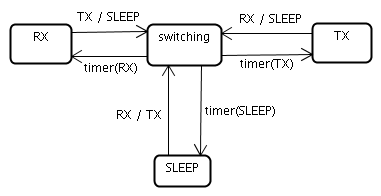
\includegraphics[width=240pt]{req_spec/stateMachineMode.png}
 % stateMachineMode.png: 1179666x1179666 pixel, 0dpi, infxinf cm, bb=
 \caption{State machine for current mode}
 \label{fig: mode state machine}
\end{figure}

\pagebreak
\subsection{send packets}

The physical layer has to be able to send packets from the MAC 
Layer to the channel. 
We also want to support the possibility to control
the sending process after it has been started.\reqdef{defsendControl}.

Before we can send packets the following things have to be 
assured:
\linebreak
\begin{itemize}
 \item the radio has to be in TX mode\reqdef{defsendPreqMode}
 \item we are not already sending\reqdef{defsendPreqSending}
 \item the channel should be idle (this is no hard requirement)\reqdef{defsendPreqIdle}
\end{itemize}

The above items should be controlled by the MAC layer so the physical layer 
would only throw an error if they are not set.

The following information has to be attached by the MAC layer to the packet:

\begin{itemize}
 \item header bitrate\reqdef{defsendCtrlHeaderBitrate}
 \item payload bitrate\reqdef{defsendCtrlBitrate}
 \item channel\reqdef{defsendCtrlChannel}
 \item TX power\reqdef{defsendCtrlTXPower}
 \item size of packet\reqdef{defsendCtrlSize}
\end{itemize}


The sending process itself is made up of the following steps:

\begin{enumerate}
 \item MAC layer gives packet and control info to physical layer\reqdef{defpacketFromMac}
 \item check requirements for sending, throw error if they are not fulfilled
 \item add information needed by the receiving physical layer to packet (see below)
 \item add signal function transmission power\footnote{The receiver converts the same signal to receiving power over time.} over time)\footnote{The signal function could be more dimensional. E.g.: receiving power over time and channel.} to packet\reqdef{defsendInfoTXPower}
 \item packet is send to channel by physical layer\reqdef{defsendToChannel}
 \item schedule transmission over message for MAC layer\reqdef{deftxover}
\end{enumerate}

The following information is needed by the receiving physical layer:

\begin{itemize}
\item TX power (represented by the signal function)\reqdef{defsendInfoTXPower}
\item position, move direction and speed of the sending host\reqdef{defsendInfoMove}
\item the channel\reqdef{defsendInfoChannel}
\item size of packet\reqdef{defsendInfoSize}
\item the duration the signal would need to be transmitted\reqdef{defsendInfoDuration}
\item the duration of the preamble\reqdef{defsendInfoPreambleDuration}
\item the bitrate (payload and header)\reqdef{defsendInfoBitrate}
\end{itemize}

\subsection{receive packets}

Because the packets arrive immediatly at every receiving node we have to simulate the receiving process:

\begin{enumerate}
\item simulate propagation delay (if needed)\reqdef{defrcvSimDelay}
\item simulate preamble duration\reqdef{defrcvSimPreamble}
\item simulate payload duration\reqdef{defrcvSimDuration}
\end{enumerate}

We also have to simulate the attenuation of the signal strength\reqdef{defrcvSimAttenuation}. This should be done by filtering the with the \textit{analogue models}.

If the preamble is transmitted the packet has to be classified as \textit{signal} or \textit{noise}\reqdef{defrcvClassify}. The decision is made by the \textit{decider}. Therefore the preamble has to be filtered previously by the analogue models.\reqdef{defrcvFilterPreamble}

If the transmission of a \textit{signal} is over we have to decide if it was received correctly.\reqdef{defrcvIsCorrect} This is also done by the \textit{decider} by evaluating the \textit{signal to noise ratio} short \textit{SNR}. Of course we have to apply the \textit{analogue model} to the signal and every noise interfering with the signal beforehand.\reqdef{defrcvFilterSignals} If the signal was received correctly we pass it to the MAC Layer.\reqdef{defrcvPassToMAC}

\subsubsection{the analogue model}

The \textit{analogue model} simulates the attenuation of the signal strength by filtering the receiving power function\reqdef{defanalogueFilter}.

There should be models to simulate the following things:

\begin{itemize}
 \item pathloss\reqdef{defanalogueSimPathloss}
 \item shadowing\reqdef{defanalogueSimShadowing}
 \item fading\reqdef{defanalogueSimFading}
\end{itemize}

Further we set the following requirements to the \textit{analogue models}:

\begin{itemize}
 \item physical layer should be able to apply multiple \textit{analogue models} to a signal\reqdef{defanalogueMulti}
 \item you should be able to set the \textit{analogue models} independent from physical layer\reqdef{defanalogueIndependent}
 \item you should be able to add your own \textit{analogue models}\reqdef{defanalogueExtensible}
\end{itemize}

\subsubsection{the decider}

As mentioned already above the \textit{decider} has to decide the following things:

\begin{itemize}
\item classify packet as signal or noise at base of the preamble\reqdef{defrcvClassify}
\item decide if a packet was received correct at base of the signal at interfering noise\reqdef{defrcvIsCorrect}
\end{itemize}

We set the following requirements to the \textit{decider}:

\begin{itemize}
 \item you should be able to set the \textit{decider} independent from physical layer\reqdef{defdeciderIndependent}
 \item you should be able to add your own \textit{decider}\reqdef{defdeciderExtensible}
 \item the \textit{decider} should be able to return bitwise correctness of the \textit{signal} (on demand)\reqdef{defdeciderBitwise}
\end{itemize}


\subsection{statistical information}

You should be able to get the following statistical information (the physical layer should not evaluate them but has to provide access to the according information):

\begin{itemize}
\item packet count\reqdef{defstatPackets}
\item received signal strength\reqdef{defstatRSS}
\item signal to noise ratio\reqdef{defstatSNR}
\item bit error ratio\reqdef{defstatBER}
\item collisions\reqdef{defstatColls}
\end{itemize}

\subsection{parameters}

The following parameters of the physical layer should be freely configurable:

\begin{itemize}
	\item simulate propagation delay? (boolean)\reqdef{defconfDelay}
	\item which analogue models should be used\reqdef{defconfAnalogue}
	\item the parameters for the analogue models\reqdef{defconfAnalogueParam}
	\item which decider should be used\reqdef{defconfDecider}
	\item the parameters for the decider\reqdef{defconfDeciderParam}
	\item thermal noise\reqdef{defconfNoise}
	\item sensitivity\reqdef{defconfSens}
	\item maximum TX power\reqdef{defconfMaxTXPower}
	\item switching times between modes (RX, TX, SLEEP)\reqdef{defconfSwitchingTimes}
\end{itemize}

\subsection{list of requirements}

\begin{enumerate}
 \item provide status information to MAC
	\begin{enumerate}
	\item provide passive (on demand) \label{provpassive}
	\item provide active (messages) \label{provactive}
	\item channelstate: idle (boolean) or RSSI \label{channelstate}
	\item current mode (RX, TX, SLEEP) \label{currentmode}
	\item transmission over event (send) \label{txover}
	\end{enumerate}
 \item switch states (RX, TX, SLEEP)
	\begin{enumerate}
	\item current mode \label{switchmode}
	\item switching times \label{switchtimes}
	\end{enumerate}
 \item send packets to air/channel
	\begin{enumerate}
	\item get packet from MAC layer\label{packetFromMac}
	\item control sending process\label{sendControl}
	\item control information needed from MAC
		\begin{enumerate}
		\item header bitrate\label{sendCtrlHeaderBitrate}
		\item payload bitrate\label{sendCtrlBitrate}
		\item channel\label{sendCtrlChannel}
		\item TX power\label{sendCtrlTXPower}
		\item size of packet\label{sendCtrlSize}
		\end{enumerate}
	\item prerequirements
		\begin{enumerate}
		\item are in TX mode \label{sendPreqMode}
		\item not already sending \label{sendPreqSending}
		\item channel is idle \label{sendPreqIdle}		
		\end{enumerate}
	\item attach informations for receiver
		\begin{enumerate}
		\item attach transmission power over time function \label{sendInfoTXPower}
		\item position, move direction and speed of the sending host \label{sendInfoMove}
		\item channel \label{sendInfoChannel}
		\item size of packet \label{sendInfoSize}
		\item duration\label{sendInfoDuration}
		\item duration of preamble \label{sendInfoPreambleDuration}
		\item bitrate (payload and header)	\label{sendInfoBitrate}
		\end{enumerate}	
	\item send to channel \label{sendToChannel}
	
	\end{enumerate}
 \item receive packets / listen for packets
		\begin{enumerate}
		\item simulate propagation delay \label{rcvSimDelay}
		\item simulate preamble \label{rcvSimPreamble}
		\item simulate transmission duration \label{rcvSimDuration}
		\item simulate attenuation \label{rcvSimAttenuation}
		\item filter preamble \label{rcvFilterPreamble}
		\item filter signal and interfering noise \label{rcvFilterSignals}
		\item pass correct packets to MAC \label{rcvPassToMAC}
		\item analogue model
			\begin{enumerate}
			\item filter signal strength \label{analogueFilter}
			\item simulate pathloss \label{analogueSimPathloss}
			\item simulate shadowing \label{analogueSimShadowing}
			\item simulate fading \label{analogueSimFading}
			\item more than one analogue model per phy \label{analogueMulti}
			\item can be set independent from phy \label{analogueIndependent}
			\item can add own analogue models \label{analogueExtensible}
			\end{enumerate}
		\end{enumerate}
		\item decider
			\begin{enumerate}
			\item classify preamble as noise or signal \label{rcvClassify}
			\item decide if packet was received correct \label{rcvIsCorrect}
			\item can be set independent from phy \label{deciderIndependent}
			\item can add own decider \label{deciderExtensible}
			\item return bitwise errors \label{deciderBitwise}
			\end{enumerate}
 \item provide hooks for statistical information
	\begin{enumerate}
	\item packet count \label{statPackets}
	\item received signal strength \label{statRSS}
	\item signal to noise ratio \label{statSNR}
	\item bit error ratio \label{statBER}
	\item collisions \label{statColls}
	\end{enumerate}
 \item configurable settings
	\begin{enumerate}
	\item simulate propagation delay? (boolean) \label{confDelay}
	\item which analogue models should be used \label{confAnalogue}
	\item the parameters for the analogue models \label{confAnalogueParam}
	\item which decider should be used \label{confDecider}
	\item the parameters for the decider \label{confDeciderParam}
	\item thermal noise \label{confNoise}
	\item sensitivity \label{confSens}
	\item maximum TX power \label{confMaxTXPower}
	\item switching times between modes (RX, TX, SLEEP) \label{confSwitchingTimes}
	\end{enumerate}
\end{enumerate}


